\documentclass{article}
\usepackage[utf8]{inputenc}
\usepackage[T1]{fontenc}
\usepackage{graphicx}
\usepackage{hyperref}
\usepackage{geometry}
\geometry{margin=1in}

\title{SWIVELS}
\date{Encyclopaedia Britannica (1771)}

\begin{document}
\maketitle

\section*{Historical source}
\textbf{Entry ID:} \texttt{entry-swivels-251} \\
\textbf{Volume ID:} 191679021 \\
\textbf{Character Count:} 1004

\subsection*{Extracted Text}
SWIVELS, a kind of ring made to turn round in a
fluids, or other ring. Theirs are ufed when a ship lies st
he monitoring sals in teleckes for adults, that they may turn
round without overwarping the tedder.

\_Switet-Canonas\_, is a fault piece of artillery belonging to
a filing of way which carries a flux of half a pound, and is
fixed in a locked on the top of the ship's ride, then, or how,
and also in her tops. The renumion of this piece are con-
tained in a fara of iron roots, of which the lowest tre-
minutes in a cylindrical pivot rolling in the locket, fo as to
fupport the weight of the canon." the footer is born in
the living place of sky, resulting with from hoops in order
to cable it to fulltain the recoil. By means of this frame,
which called the \_hybrid\_, and as iron heads on its caf-
sible, the game be directed by the head to any object.
It is therefore very necellary in the tops, particularly when
loaded with multiclusls, to fire down on the upper decks
of the shelter in an area.



\section*{Source record}
\begin{itemize}
\item \textbf{Dataset:} \texttt{NationalLibraryOfScotland/encyclopaedia\_britannica\_illustrated}
\item \textbf{Dataset Revision:} \texttt{309f765b1ecc83e0a7f7762e44b4a927a7555443}
\item \textbf{Page ID:} \texttt{britannica:309f765b1ecc83e0a7f7762e44b4a927a7555443:train:251} \\
  \textbf{Filename:} \texttt{page-0251-69952e7c4a0f.jpg} \\
  \textbf{Row Index:} 251 \\
  \textbf{SHA256:} \texttt{69952e7c4a0f4026...}
\end{itemize}

\begin{figure}[h]
\centering
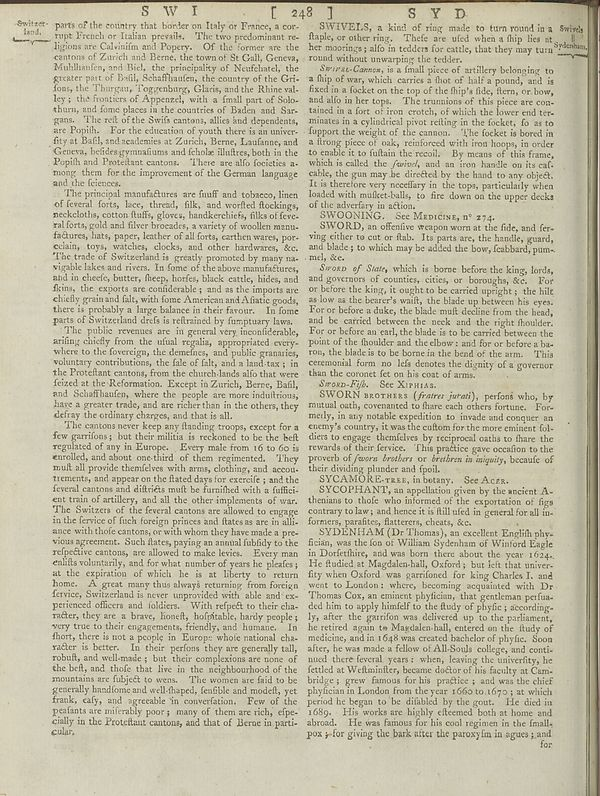
\includegraphics[width=0.85\textwidth]{../scans/page-0251-69952e7c4a0f.jpg}
\caption*{Source scan: \texttt{page-0251-69952e7c4a0f.jpg}}
\end{figure}

\end{document}
